\newsection{Pianificazione}
In riferimento alle scadenze elencate nella sottosezione 1.5, abbiamo suddiviso lo sviluppo del progetto in cinque macro-fasi:
\begin{itemize}
\item{Analisi;}
\item{Consolidamento dei Requisiti;}
\item{Progettazione Architetturale;}
\item{Progettazione di Dettaglio e Codifica;}
\item{Verifica e \gl{Validazione}.}
\end{itemize}

Abbiamo suddiviso ogni macro-periodo in attività da svolgere durante il periodo specifico, le quali a loro volta sono state scomposte in sotto-attività ancor più di dettaglio. Le sotto-attività sono riportate unicamente nel Gantt. \\ Nel Gantt le attività sono individuate dal colore blu, salvo l'attività di finale verifica che è stata contrassegnata con il colore verde. Inoltre, vengono riportate:
\begin{itemize}
\item{\gl{Milestone}: data attesa di conclusione delle attività, indicata nel Gantt con un rombo rosso;}
\item{Attività singola: attività principale suddivisa in sotto-attività, indicata nel Gantt con una barra nera.}
\end{itemize}

\subsection{Analisi}

\subsubsection{Prospetto Orario}
Nel periodo di analisi la distribuzione oraria è la seguente:

\renewcommand{\arraystretch}{1.5}
\begin{table}[H]
\begin{center}
\begin{tabular}{|c|c|c|c|c|c|c|c|}
\hline
\rowcolor{title_row}
\textbf{\color{title_text}{Nome}} & \textbf{\color{title_text}{Resp.}} & \textbf{\color{title_text}{Ammi.}} & \textbf{\color{title_text}{Analist.}} & \textbf{\color{title_text}{Progett.}} & \textbf{\color{title_text}{Program.}} & \textbf{\color{title_text}{Verific.}} & \textbf{\color{title_text}{Totale}} \\ \hline
Andrea Trevisin  & 6 & 2 & 10 & & & 6 & 24  \\ \hline
Giacomo Barzon   & 4 & 3 & 12 & & & 4 & 23  \\ \hline
Giovanni Sorice  & & 3 & 14 & & & 5 & 22  \\ \hline
Lorenzo Busin    & & 8 & 8 & & & 6 & 22  \\ \hline
Marco Costantino & 5 & 5 & 10 & & & 3 & 23 \\ \hline
Michele Roverato & 9 & 4 & 7 & & & 2 & 22 \\ \hline
Nicolò Tartaggia & 5 & & 8 & & & 10 & 23  \\ \hline
\end{tabular}
\caption{Tabella 5.1.1: Distribuzione oraria del periodo "Analisi"\label{}}
\end{center}
\end{table}
\renewcommand{\arraystretch}{1}

Il seguente grafico dà una rappresentazione visiva della suddivisione oraria: \\
\begin{center}
//Grafico
\end{center}


\subsubsection{Prospetto Economico}
Nel periodo di analisi il resoconto della distribuzione delle ore e dei relativi costi è la seguente:

\renewcommand{\arraystretch}{1.5}
\begin{table}[H]
\begin{center}
\begin{tabular}{|c|c|c|}
\hline
\rowcolor{title_row}
\textbf{\color{title_text}{Ruolo}}  & \textbf{\color{title_text}{Ore}} & \textbf{\color{title_text}{Costo in \euro}} \\ \hline
Responsabile    & 29           & 870                 \\ \hline
Amministratore  & 25           & 500                 \\ \hline
Analista        & 69           & 1725                \\ \hline
Progettista     &              &                     \\ \hline
Programmatore   &              &                     \\ \hline
Verificatore    & 36           & 540                 \\ \hline
\textbf{Totale} & \textbf{159}    & \textbf{3635}    \\ \hline
\end{tabular}
\caption{Tabella 5.1.2: Prospetto economico del periodo "Analisi"\label{}}
\end{center}
\end{table}
\renewcommand{\arraystretch}{1}

Il seguente grafico dà una rappresentazione visiva della distribuzione dei ruoli: \\
\begin{center}
//Grafico
\end{center}

\pagebreak

\subsection{Consolidamento dei requisiti}

\subsubsection{Prospetto orario}
Nel periodo di consolidamento dei requisiti la distribuzione oraria è la seguente:

\renewcommand{\arraystretch}{1.5}
\begin{table}[H]
\begin{center}
\begin{tabular}{|c|c|c|c|c|c|c|c|}
\hline
\rowcolor{title_row}
\textbf{\color{title_text}{Nome}} & \textbf{\color{title_text}{Resp.}} & \textbf{\color{title_text}{Ammi.}} & \textbf{\color{title_text}{Analist.}} & \textbf{\color{title_text}{Progett.}} & \textbf{\color{title_text}{Program.}} & \textbf{\color{title_text}{Verific.}} & \textbf{\color{title_text}{Totale}} \\ \hline
Andrea Trevisin  & 5 & 2 & & & & & 7 \\ \hline
Giacomo Barzon   & & & 3 & & & 3 & 6 \\ \hline
Giovanni Sorice  & & 5 & & & & 1 & 6 \\ \hline
Lorenzo Busin    & 5 & 1 & 4 & & & & 10 \\ \hline
Marco Costantino & & & 3 & & & 5 & 8 \\ \hline
Michele Roverato & & & 3 & & & 5 & 8 \\ \hline
Nicolò Tartaggia & & 3 & & & & 5 & 8 \\ \hline
\end{tabular}
\caption{Tabella 5.2.1: Distribuzione oraria del periodo "Consolidamento dei requisiti"\label{}}
\end{center}
\end{table}
\renewcommand{\arraystretch}{1}

Il seguente grafico dà una rappresentazione visiva della suddivisione oraria: \\
\begin{figure} [H]
	\centering
	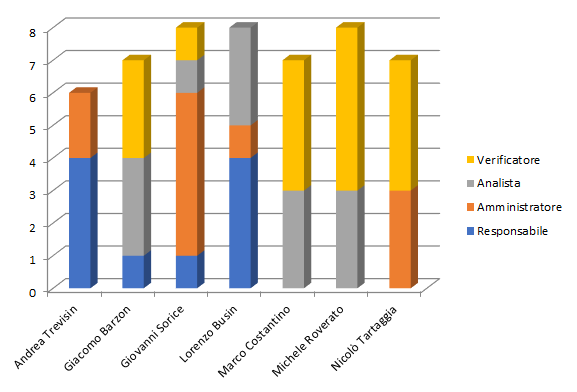
\includegraphics[scale=1]{Res/ExcelGrafici/Grafici/ConsolidamentoOre.png}
	\caption{Figura 5.2.1: Grafico suddivisione oraria del periodo "Consolidamento dei requisiti"}\label{}
\end{figure}


\subsubsection{Prospetto economico}
Nel periodo di consolidamento dei requisiti il resoconto della distribuzione delle ore e dei relativi costi è la seguente:

\renewcommand{\arraystretch}{1.5}
\begin{table}[H]
\begin{center}
\begin{tabular}{|c|c|c|}
\hline
\rowcolor{title_row}
\textbf{\color{title_text}{Ruolo}}  & \textbf{\color{title_text}{Ore}} & \textbf{\color{title_text}{Costo in \euro}} \\ \hline
Responsabile    & 10 & 300 \\ \hline
Amministratore  & 11 & 220 \\ \hline
Analista        & 13 & 325 \\ \hline
Progettista     & & \\ \hline
Programmatore   & & \\ \hline
Verificatore    & 19 & 285 \\ \hline
\textbf{Totale} & \textbf{53}    & \textbf{1.130}    \\ \hline
\end{tabular}
\caption{Tabella 5.2.2: Prospetto economico del periodo "Consolidamento dei requisiti"\label{}}
\end{center}
\end{table}
\renewcommand{\arraystretch}{1}

Il seguente grafico dà una rappresentazione visiva della distribuzione dei ruoli: \\
\begin{figure} [H]
	\centering
	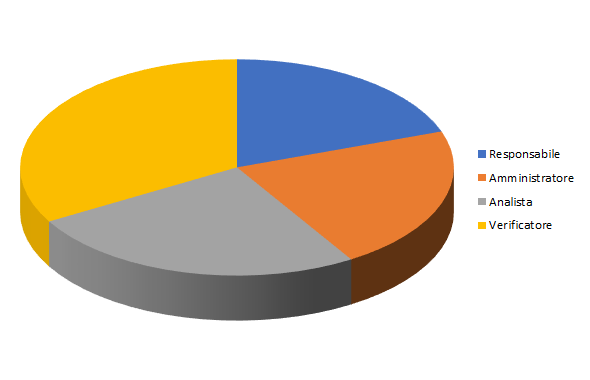
\includegraphics[scale=1]{Res/ExcelGrafici/Grafici/ConsolidamentoRuoli.png}
	\caption{Figura 5.2.2: Grafico suddivisione dei ruoli del periodo "Consolidamento dei requisiti"}\label{}
\end{figure}

\pagebreak

\subsection{Progettazione architetturale}

\subsubsection{Prospetto Orario}
Nel periodo di progettazione architetturale la distribuzione oraria è la seguente:

\renewcommand{\arraystretch}{1.5}
\begin{table}[H]
\begin{center}
\begin{tabular}{|c|c|c|c|c|c|c|c|}
\hline
\rowcolor{title_row}
\textbf{\color{title_text}{Nome}} & \textbf{\color{title_text}{Resp.}} & \textbf{\color{title_text}{Ammi.}} & \textbf{\color{title_text}{Analist.}} & \textbf{\color{title_text}{Progett.}} & \textbf{\color{title_text}{Program.}} & \textbf{\color{title_text}{Verific.}} & \textbf{\color{title_text}{Totale}} \\ \hline
Andrea Trevisin  & & & & 14 & 6 & 12 & 32 \\ \hline
Giacomo Barzon   &  & 4 &  & 10 & 8 & 8 & 30\\ \hline
Giovanni Sorice  & 8 &  &  & 10 & 6 & 8 & 32\\ \hline
Lorenzo Busin    &  & 3  &  & 12 & 8 & 10 & 33\\ \hline
Marco Costantino & 6 &  &  &  & 10 & 14 & 30\\ \hline
Michele Roverato &  & 6 & 8 &  & 8 & 10 & 32\\ \hline
Nicolò Tartaggia &  & 5  & 8 &  & 10 & 8 & 31\\ \hline
\end{tabular}
\caption{Tabella 5.3.1: Distribuzione oraria del periodo "Progettazione architetturale"\label{}}
\end{center}
\end{table}
\renewcommand{\arraystretch}{1}

Il seguente grafico dà una rappresentazione visiva della suddivisione oraria: \\
\begin{figure} [H]
	\centering
	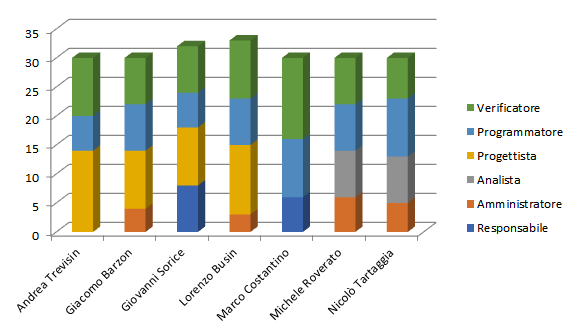
\includegraphics[scale=1]{Res/ExcelGrafici/Grafici/ProgettazioneOre.png}
	\caption{Figura 5.3.1: Grafico suddivisione oraria del periodo "Progettazione architetturale"}\label{}
\end{figure}


\subsubsection{Prospetto Economico}
Nel periodo di progettazione architetturale il resoconto della distribuzione delle ore e dei relativi costi è la seguente:

\renewcommand{\arraystretch}{1.5}
\begin{table}[H]
\begin{center}
\begin{tabular}{|c|c|c|}
\hline
\rowcolor{title_row}
\textbf{\color{title_text}{Ruolo}}  & \textbf{\color{title_text}{Ore}} & \textbf{\color{title_text}{Costo in \euro}} \\ \hline
Responsabile    & 14              & 420                     \\ \hline
Amministratore  & 18              & 360                   \\ \hline
Analista        & 16              & 400                    \\ \hline
Progettista     & 46              & 1.012                     \\ \hline
Programmatore   & 56              & 840                     \\ \hline
Verificatore    & 70              & 1.050                    \\ \hline
\textbf{Totale} & \textbf{220}    & \textbf{4.082}         \\ \hline
\end{tabular}
\caption{Tabella 5.3.2: Prospetto economico del periodo "Progettazione architetturale"\label{}}
\end{center}
\end{table}
\renewcommand{\arraystretch}{1}

Il seguente grafico dà una rappresentazione visiva della distribuzione dei ruoli: \\
\begin{figure} [H]
	\centering
	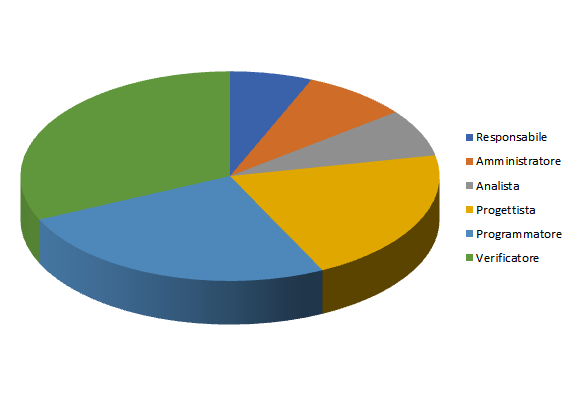
\includegraphics[scale=1]{Res/ExcelGrafici/Grafici/ProgettazioneRuoli.png}
	\caption{Figura 5.3.2: Grafico suddivisione dei ruoli del periodo "Progettazione architetturale"}\label{}
\end{figure}

\pagebreak

\subsection{Periodo di progettazione di dettaglio e codifica}
\subsubsection{Consuntivo}
\renewcommand{\arraystretch}{1.5}
\begin{table}[H]
\begin{center}
\begin{tabular}{|c|c|c|c|c|c|c|c|}
\hline
\rowcolor{title_row}
\textbf{\color{title_text}{Nome}} & \textbf{\color{title_text}{Resp.}} & \textbf{\color{title_text}{Ammi.}} & \textbf{\color{title_text}{Analist.}} & \textbf{\color{title_text}{Progett.}} & \textbf{\color{title_text}{Program.}} & \textbf{\color{title_text}{Verific.}} & \textbf{\color{title_text}{Totale}} \\ \hline
Andrea Trevisin  & & 8 & & 10 & 19 & 16 & 53 \\ \hline
Giacomo Barzon   & 4 & 5 & & 11 & 19 & 16 & 55  \\ \hline
Giovanni Sorice  & 6 & & & 12 & 20 & 14 & 52 \\ \hline
Lorenzo Busin    & 7 & 3 & & 13 & 19 & 13 & 55 \\ \hline
Marco Costantino & & & 5 & 14 & 20 & 15 & 54 \\ \hline     
Michele Roverato & & 4 & & 11 & 22 & 15 & 52 \\ \hline    
Nicolò Tartaggia & & & 5 & 10 & 21 & 17 & 53 \\ \hline
\end{tabular}
\caption{Tabella 6.1.1(1): Resoconto orario delle ore effettivamente impiegate dai membri del team nel periodo "Progettazione architetturale"\label{}}
\end{center}
\end{table}
\renewcommand{\arraystretch}{1}

\renewcommand{\arraystretch}{1.4}
\begin{table}[H]
\begin{center}
\begin{tabular}{|c|c|c|c|}
\hline
\rowcolor{title_row}
\textbf{\color{title_text}{Ruolo}}  & \textbf{\color{title_text}{Ore}} & \textbf{\color{title_text}{Costo in \euro}} & \textbf{\color{title_text}{Differenza al preventivo in \euro}} \\ \hline
Responsabile    & 17 & 510 & \\  \hline
Amministratore  & 10 (-10)& 200 & -100 \\ \hline
Analista        & 5 (-5) & 125 & -125 \\ \hline
Progettista     & 88 (+7) & 1.936 & +154\\ \hline
Programmatore   & 140 (+5) & 2.175 & +75\\ \hline
Verificatore    & 121 (+15) & 1.815& +225\\ \hline
\textbf{Totale} & \textbf{374 (+12)}    & \textbf{6861} & \textbf{+229} \\ \hline
\end{tabular}
\caption{Tabella 6.1.1(2): Resoconto economico delle ore effettivamente impiegate per ogni ruolo nel periodo "Progettazione architetturale"\label{}}
\end{center}
\end{table}
\renewcommand{\arraystretch}{1}


\subsubsection{Variazioni dalla pianificazione}
// TO BE DONE

\subsubsection{Considerazioni}
// TO BE DONE
\pagebreak

\subsection{Verifica e validazione}

\subsubsection{Prospetto orario}
Nel periodo di verifica e validazione la distribuzione oraria è la seguente:

\renewcommand{\arraystretch}{1.5}
\begin{table}[H]
\begin{center}
\begin{tabular}{|c|c|c|c|c|c|c|c|}
\hline
\rowcolor{title_row}
\textbf{\color{title_text}{Nome}} & \textbf{\color{title_text}{Resp.}} & \textbf{\color{title_text}{Ammi.}} & \textbf{\color{title_text}{Analist.}} & \textbf{\color{title_text}{Progett.}} & \textbf{\color{title_text}{Program.}} & \textbf{\color{title_text}{Verific.}} & \textbf{\color{title_text}{Totale}} \\ \hline
Andrea Trevisin  & & 6 & & & 7 & 7 & 20  \\ \hline
Giacomo Barzon   & & & & 7 & 6 & 7 & 20  \\ \hline
Giovanni Sorice  & & 8 & &  & 6 & 7 & 21  \\ \hline
Lorenzo Busin    & & & & & 7 & 10 & 17  \\ \hline
Marco Costantino & & 7 & & & 7 & 7 & 21  \\ \hline
Michele Roverato & & & & 7 & 7 & 7 & 21  \\ \hline
Nicolò Tartaggia & 10 & & & 6 & 5 & & 21  \\ \hline
\end{tabular}
\caption{Tabella 5.5.1: Distribuzione oraria del periodo "Verifica e validazione"\label{}}
\end{center}
\end{table}
\renewcommand{\arraystretch}{1}

Il seguente grafico dà una rappresentazione visiva della suddivisione oraria: \\
\begin{figure} [H]
	\centering
	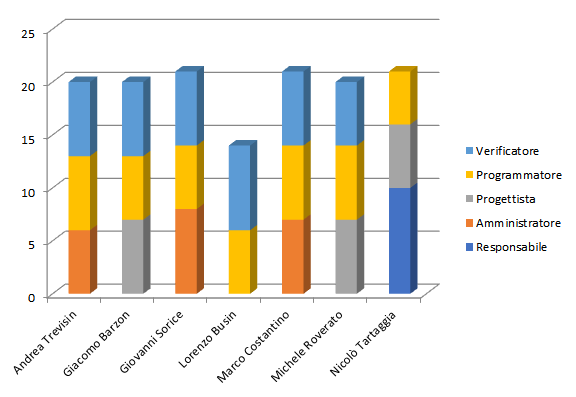
\includegraphics[scale=1]{Res/ExcelGrafici/Grafici/VerificaOre.png}
	\caption{Figura 5.5.1: Grafico suddivisione oraria del periodo "Verifica e validazione"}\label{}
\end{figure}


\subsubsection{Prospetto economico}
Nel periodo di verifica e validazione il resoconto della distribuzione delle ore e dei relativi costi è la seguente:

\renewcommand{\arraystretch}{1.5}
\begin{table}[H]
\begin{center}
\begin{tabular}{|c|c|c|}
\hline
\rowcolor{title_row}
\textbf{\color{title_text}{Ruolo}}  & \textbf{\color{title_text}{Ore}} & \textbf{\color{title_text}{Costo in \euro}} \\ \hline
Responsabile    & 10 & 300 \\ \hline
Amministratore  & 21 & 420 \\ \hline
Analista        & & \\ \hline
Progettista     & 20 & 440 \\ \hline
Programmatore   & 45 & 675 \\ \hline
Verificatore    & 45 & 675 \\ \hline
\textbf{Totale} & \textbf{141}    & \textbf{2.510}           \\ \hline
\end{tabular}
\caption{Tabella 5.5.2: Prospetto economico del periodo "Verifica e validazione"\label{}}
\end{center}
\end{table}
\renewcommand{\arraystretch}{1}

Il seguente grafico dà una rappresentazione visiva della distribuzione dei ruoli: \\
\begin{figure} [H]
	\centering
	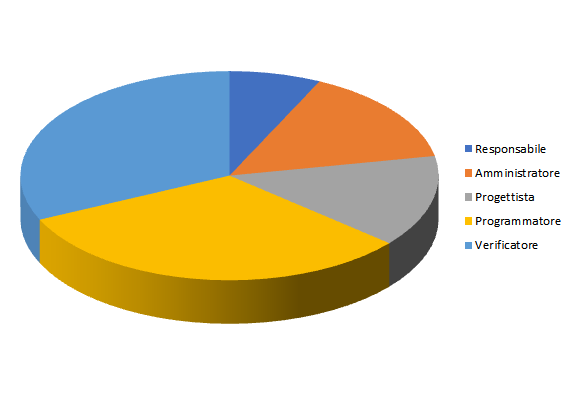
\includegraphics[scale=1]{Res/ExcelGrafici/Grafici/VerificaRuoli.png}
	\caption{Figura 5.5.2: Grafico suddivisione dei ruoli del periodo "Verifica e validazione"}\label{}
\end{figure}

\pagebreak

\pagebreak
